\chapter{\uppercase{Placa electrònica d'adquisició de dades i comunicació}}
Tal com s'indica als objectius del projecte part del treball consisteix en desenvolupar una placa electrònica encarregada d'adquirir dades, en aquest cas de tensió, dels panells fotovoltaics.\\
\newline Es vol que aquestes dades siguin accessibles i per això s'ha optat per dotar la placa d'un component de comunicació Wi-Fi gràcies al qual es podrà visualitzar una pàgina web amb les dades mesurades.\\
\newline La placa disposa d'una part d'alimentació que s'encarrega d'adaptar les tensions als nivells correctes dels diversos components. Uns circuits d'instrumentació atenuen la tensió d'entrada i fan les restes per obtenir la diferència de tensió entre els dos terminals de cada panell. Es multiplexen les senyals i es llegeix el seu valor digital.

\section{Alimentació}
% Comentar com s'aliment placaa la. Afegir l'equip a amidaments i pressupost.
La placa dissenyada s'alimenta amb un cable Micro-USB el qual es connecta a un equip de potència format per un rectificador i un convertidor DC-DC reductor, o sigui, de tipus Buck. Aquest equip, que molta gent identificaria com un carregador de telèfon mòbil, entrega 5 V a la seva sortida i un màxim de 2 A.\\
\newline La placa electrònica dissenyada disposa d'un integrat SMD que converteix la tensió de 5 V a 3,3 V, anomenat SPX3819M5-L-3-3. Els operacionals van alimentats a 5 V. L'integrat de comunicacions i altres parts de la placa van alimentats amb 3,3 V.\\
\newline Algunes característiques del regulador són les indicades a la Taula \ref{tab:regulador}.
\begin{table}[H]
\small
\begin{center}
 \begin{tabular} {|l|r|}%{X | c c c} 
 \hline
 Característica & Valor \\
 \hline \hline 
Tensió de sortida & 3,3 V \\ \hline
Corrent màxim de sortida & 500 mA\\ \hline
Tensió mínima d'entrada & 2,5 V \\ \hline
Precisió de regulació de voltatge & 1\% \\ \hline
Tensió màxima d'entrada & 16 V \\ \hline
Corrent de repòs & 90 $\mu$A \\ \hline
Empaquetat & SOT-23-5 \\ \hline

 \end{tabular}
 \caption{Característiques del regulador de tensió SPX3819M5-L-3-3}
 \label{tab:regulador}
\end{center}
\end{table}
%\si\ohm

\noindent Pel que fa a la intensitat, la placa consumeix al voltant de 100 mA en funcionament normal. Pot arribar a consumir uns 200 mA en certs moments. El convertidor de tensió de 5 V a 3,3 V pot donar fins a 500 mA a la seva sortida, molt superior al màxim que pot necessitar la placa.\\
\newline L'esquema de connexionat del regulador és el de la Figura \ref{fig: circuit_reg}.
\begin{figure}[H]
\begin{center}
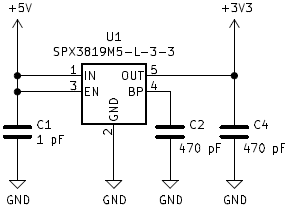
\includegraphics[scale=0.5]{images/regulador.png}
\end{center}
\caption{Regulador de tensió}
\label{fig: circuit_reg}

\end{figure}
\noindent El convertidor de tensió disposa de condensadors a l'entrada i a la sortida per tal de garantir una tensió el més constant possible, per bé que la recomanació del fabricant és connectar-ne només un a l'entrada. Si la sortida sol·licita un pic de corrent els condensadors el poden subministrar durant els instants en què el regulador encara no hagi reaccionat.\\
\newline Així, el dimensionament dels equips d'alimentació es considera correcte.

\section{Instrumentació}
% Insistir en la part d'instrumentació, posar equacions i indicar càlculs seguits
% Discutir per què s'ha escollit un OP AMP o un altre i així
La placa disposa d'una part d'instrumentació que s'encarrega d'adaptar les tensions dels panells solars fotovoltaics a les tensions amb què pot treballar el convertidor analògic digital. Interessa conèixer la diferència de tensió als terminals de cada placa. El circuit és l'indicat a la Figura \ref{fig:restador}.\\
\newline El primer que es fa és reduir la tensió considerablement mitjançant un divisor de tensió connectat a un seguidor de voltatge. El seguidor de voltatge és important tenir-lo per aïllar aquesta primera etapa de la resta. Les resistències es detallen a l'estat d'amidaments i al pressupost. El seu valor de potència màxima a dissipar és adient.\\
\newline El divisor de tensió ha de ser tal faci que a l'entrada no inversora la tensió sigui menor o igual a 3,5 V, tal com s'exposa més endavant.

\begin{figure}[H]
\begin{center}
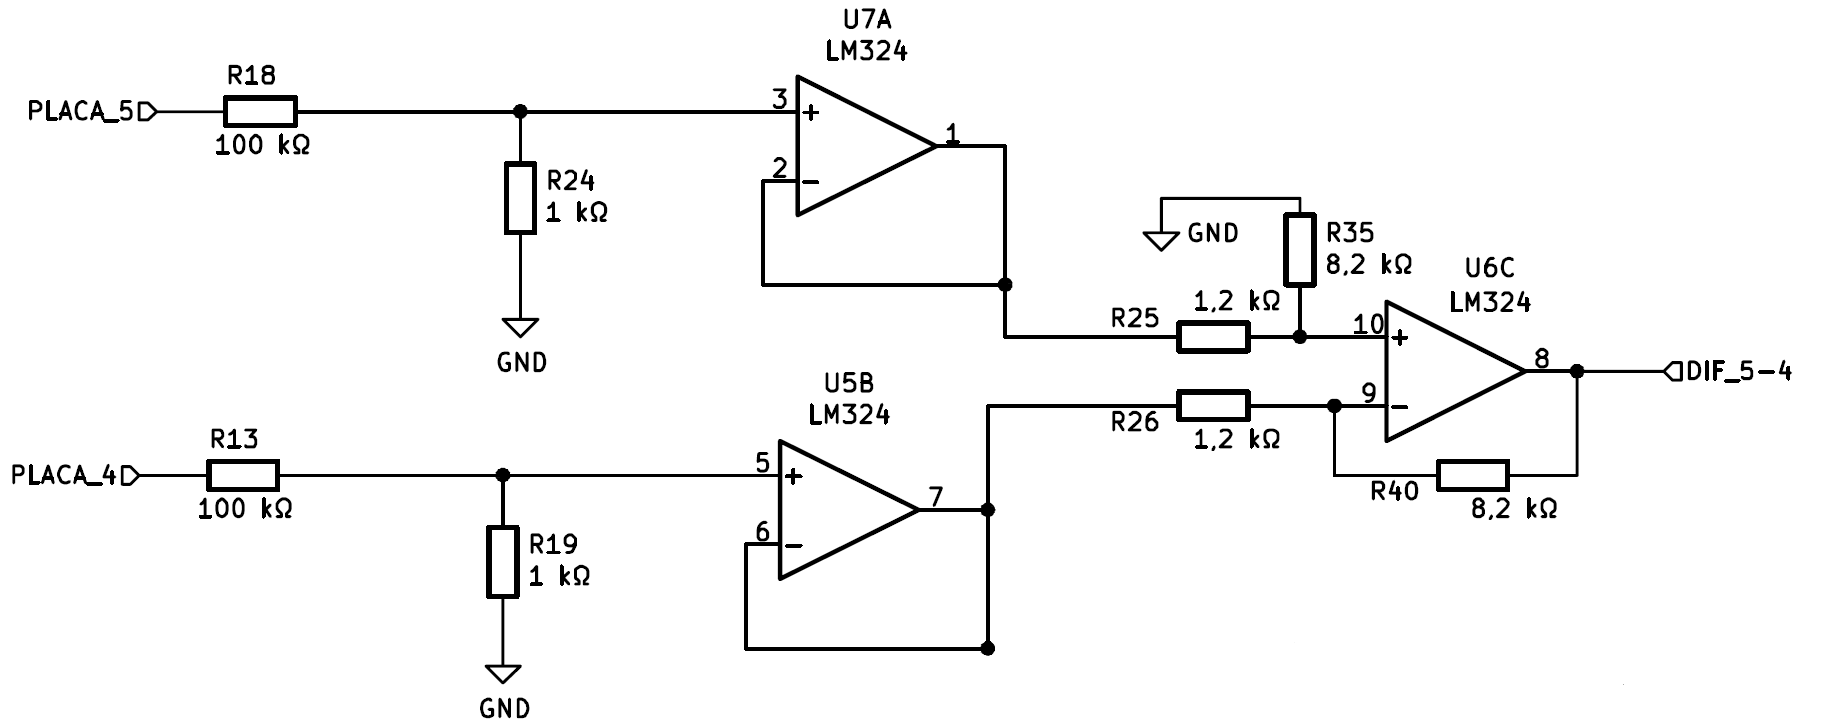
\includegraphics[scale=0.3]{images/restador.png}
\end{center}
\caption{Circuit atenuador i restador}
\label{fig:restador}
\end{figure}

\noindent El guany de la primera etapa és el de l'Equació \ref{guany1}.

\begin{equation} \label{guany1}
\Delta_{1}=\frac{R_{24}}{R_{24}+R_{18}}
\end{equation}

\noindent Seguidament s'utilitza un restador que alhora amplifica la tensió resultant. El fabricant de les plaques ens dona un màxim de tensió de 46,2 V que per efectes de la temperatura pot passar a valer 51,37 V. Tenim en compte aquesta tensió per dimensionar el restador. El circuit està dissenyat per aprofitar tot el rang del convertidor analògic digital.\\
\newline S'imposa que els parells següents de resistències siguin iguals, per simplificar els càlculs. La primera parella de resistències iguals són la de l'Equació \ref{r1}.

\begin{equation} \label{r1}
R_{25}=R_{26}
\end{equation}

\noindent I el mateix per l'altre parell, segons l'Equació \ref{r2}.
\begin{equation} \label{r2}
R_{35}=R_{40}
\end{equation}

\noindent Aleshores el guany de la segona etapa ve donat per l'Equació \ref{guany2}.

\begin{equation} \label{guany2}
\Delta_{2}=\frac{R_{35}}{R_{25}}
\end{equation}

\noindent Aquest guany és de 6,8. Amb tot això podem escriure la relació entre les dues entrades i la sortida del circuit mostrat. Ho indica l'Equació \ref{relacio}.
\begin{equation} \label{relacio}
V_{5-4} =  \left (V_5 - V_4  \right ) \Delta_{1} \Delta_{2} = 0,0677
\end{equation}


%
%
%
\noindent Els amplificadors operacions escollits són del model LM324. Són de baix cost i les seves prestacions són més que suficients per aquest cas en què es treballa amb senyals contínues. Algunes característiques s'indiquen a la Taula \ref{tab:lm324}.
\begin{table}[H]
\small
\begin{center}
 \begin{tabular} {|l|r|}%{X | c c c} 
 \hline
 Característica & Valor \\
 \hline \hline 
Guany unitari & 100 dB \\ \hline
Rang de tensió d'alimentació single supply & 3 V a 32 V \\ \hline
Tensió d'offset màxima & 2 mV \\ \hline
Rang de tensió de sortida & 0 V a $V_{cc}$-1,5 V \\ \hline
Corrent màxim de sortida en source & 40 mA \\ \hline

 \end{tabular}
 \caption{Característiques de l'amplificador operacional LM324}
 \label{tab:lm324}
\end{center}
\end{table}
%\si\ohm
%
\noindent El rang d'alimentació i el rang de tensió de sortida són dos paràmetres que s'han tingut molt en compte pel disseny. L'amplificador operacional LM324, tot i no ser Rail-to-Rail, l'alimentarem a 5 V i així tindrem sortides màximes de fins a 3,5 V, que és un nivell de tensió adequat per aquesta placa. El corrent de sortida i l'offset de tensió també són acceptables per l'aplicació.

\section{Multiplexor}

La placa que s'ha dissenyat disposa de l'integrat ESP-12E, que entre d'altres té una entrada analògica. Al tenir 10 senyals analògiques per llegir i una sola entrada analògica s'opta per utilitzar un multiplexor.\\
\newline Aquest multiplexor té 16 entrades, un pin per habilitar-lo, 4 pins per seleccionar quin canal llegir i una sola sortida.\\
\newline Tot i que els multiplexors són molt usats en electrònica digital, el fabricant ens indica que també està pensat per fer servir amb senyals analògiques, gràcies a la baixa resistència entre una entrada habilitada i la sortida.\\
\newline El multiplexor i la connexió de la sortida analògica al mòdul ESP-12E és la indicada a la Figura \ref{fig:mux}.\\
\newline Cal dir que aquesta imatge és una simplificació del circuit mostrat a plànols. S'han eliminat algunes connexions per fer la figura més entenedora.

\begin{figure}[H]
\begin{center}
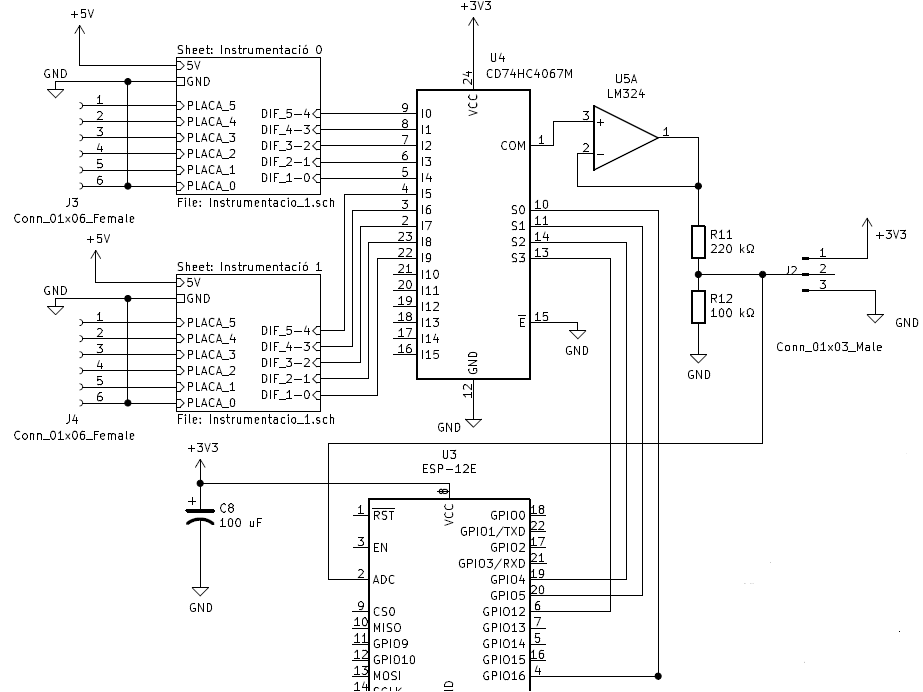
\includegraphics[scale=0.60]{images/mux.png}
\end{center}
\caption{Multiplexor i entrada digital}
\label{fig:mux}
\end{figure}

\noindent Les sortides dels circuits d'instrumentació són les entrades del multiplexor. La lògica és positiva. S0 és el bit de menys pes i S3 el de més pes. S'habilita el multiplexor connectant-lo a massa.\\
\newline Per la programació, no s'ha de confondre l'etiqueta del component ESP-12E amb el número de pin que es programarà. Això es pot visualitzar a la Taula \ref{tab:programacio_pins}.

\begin{table}[H]
\small
\begin{center}
 \begin{tabular} {|l|r|}%{X | c c c} 
 \hline
 GPIO & Número de pin a programar  \\ \hline \hline 
GPIO 12 & 6 \\ \hline
GPIO 4 & 2 \\ \hline
GPIO 5 & 1 \\ \hline
GPIO 16 & 0 \\ \hline
 \end{tabular}
 \caption{Relació entre les sortides i el seu número de pin a programar}
 \label{tab:programacio_pins}
\end{center}
\end{table}

\noindent Com s'indica a l'annex de programació, es programen els pins de caràcter general com a sortides per controlar el multiplexor.\\
\newline La taula de veritat és la de la Taula \ref{tab:veritat}.

\begin{table}[H]
\small
\begin{center}
 \begin{tabular} {|l|l|l|l|l|r|}%{X | c c c} 
 \hline
 CGPIO12 & GPIO4 & GPIO5 & GPIO16 & ~E & Sortida \\ \hline \hline 
 0 & 0 & 0 & 0 & 0 & 0\_DIF\_5-4 \\ \hline
 0 & 0 & 0 & 1 & 0 & 0\_DIF\_4-3 \\ \hline
 0 & 0 & 1 & 0 & 0 & 0\_DIF\_3-2 \\ \hline
 0 & 0 & 1 & 1 & 0 & 0\_DIF\_2-1 \\ \hline
 0 & 1 & 0 & 0 & 0 & 0\_DIF\_1-0 \\ \hline
 
 0 & 1 & 0 & 1 & 0 & 1\_DIF\_5-4 \\ \hline
 0 & 1 & 1 & 0 & 0 & 1\_DIF\_4-3 \\ \hline
 0 & 1 & 1 & 1 & 0 & 1\_DIF\_3-2 \\ \hline
 1 & 0 & 0 & 0 & 0 & 1\_DIF\_2-1 \\ \hline
 1 & 0 & 0 & 1 & 0 & 1\_DIF\_1-0 \\ \hline
 \end{tabular}
 \caption{Taula de veritat}
 \label{tab:veritat}
\end{center}
\end{table}

\noindent Algunes característiques del multiplexor són les de la Taula \ref{mux_ds}.
%
\begin{table}[H]
\small
\begin{center}
 \begin{tabular} {|l|r|}%{X | c c c} 
 \hline
 Característica & Valor \\
 \hline \hline 
Resistència ON, $V_{CC}$=4,5V & 70 \si\ohm \\ \hline
Rang de tensió d'alimentació & -0,5 V a 7 V \\ \hline
Temps de transició màxim & 1.000 ms \\ \hline
Corrent màxim de fuga a les entrades lògiques & 1 $\mu$A \\ \hline
Nivell lògic alt, $V_{CC}$=4,5V & 2 V \\ \hline
Nivell lògic baix, $V_{CC}$=4,5V & 0,8 V \\ \hline
 \end{tabular}
 \caption{Característiques del multiplexor CD74HC4067M}
 \label{mux_ds}
\end{center}
\end{table}



\noindent Hi ha un seguidor per tal d'aïllar les etapes i un divisor de tensió encarregat d'adaptar la tensió al conversor analògic digital, que té un màxim d'1 V. 


\section{Comunicació}
% Explicar els diferents blocs lògics de la placa
La placa electrònica dissenyada permet establir comunicació Wi-Fi de forma efectiva. L'integrat ESP-12E és un component molt popular que es basa en l'ESP8266. L'ESP-12E és un component que disposa d'una petita memòria on es bolca el programa, d'uns quants pins digitals de propòsit general, d'una entrada analògica i d'una antena impresa en circuit imprès, a més de l'ESP8266.\\
\newline El fabricant indica que es deixi una àrea lliure de coure sota l'antena per evitar interferències i problemes de comunicació.\\
\newline Tot i tenir una simple antena impresa en circuit imprès el rang de comunicació Wi-Fi és generós i suficient per l'aplicació que es desitja.\\
\newline Algunes característiques de l'ESP8266 venen donades a la Taula \ref{tab:ESP8266}.
\begin{table}[H]
\small
\begin{center}
 \begin{tabular} {|l|r|}%{X | c c c} 
 \hline
 Característica & Valor \\
 \hline \hline 
Certificació & Wi-Fi Alliance \\ \hline
Freqüència de treball & 2,4 GHz \\ \hline
Potència de l'emissor & 17 dBm \\ \hline
Llindar de potència del receptor & -75 dBm \\ \hline
Rang de tensió d'alimentació & 2,5 V a 3,6 V \\ \hline
Corrent en funcionament normal & 80 mA \\ \hline

 \end{tabular}
 \caption{Característiques de l'integrat de comunicació ESP-8266}
 \label{tab:ESP8266}
\end{center}
\end{table}
% \si\ohm

\noindent D'aquí la importància d'alimentar-lo amb 3,3 V enlloc dels 5 V que ens arriben al connector. Per això es fa servir el regulador de tensió. El consum del dispositiu no és molt elevat però és considerable, no seria viable tenir la placa amb una bateria.

\section{Circuit imprès}
% Questions de PCB, clearance i tal
S'ha dissenyat un PCB a doble cara que conté la part d'alimentació, la part d'instrumentació i la part de comunicació. Disposa dels connectors necessaris.\\
\newline Les pistes d'alimentació s'han fet més gruixudes que les de senyal digital. Les pistes de tensió de les plaques s'han fet una mica més gruixudes, tot i que la intensitat a través seu és petita. La separació d'una d'aquestes pistes amb la resta és generosa per evitar l'arc elèctric. A més, es preveu recobrir la placa amb una pel·lícula, cosa que disminuiria encara més el risc d'arc elèctric.\\
\newline La majoria de components són SMD. Solen ser més barats i ocupen molt menys espai en comparació als components que travessen la placa. Així, les dimensions finals de la placa són de 8,4 x 10 cm aproximadament.\\
\newline S'han seguit especificacions del fabricant pel disseny de la part de RF. Pel disseny de la part d'instrumentació s'ha tingut especial cura en utilitzar condensadors de desacoblament a les alimentacions dels integrats i situar-los prop d'aquests.\\
\newline La vista superior de com quedaria la placa és la de la Figura \ref{fig:3d_sup}.
\begin{figure}[H]
\begin{center}
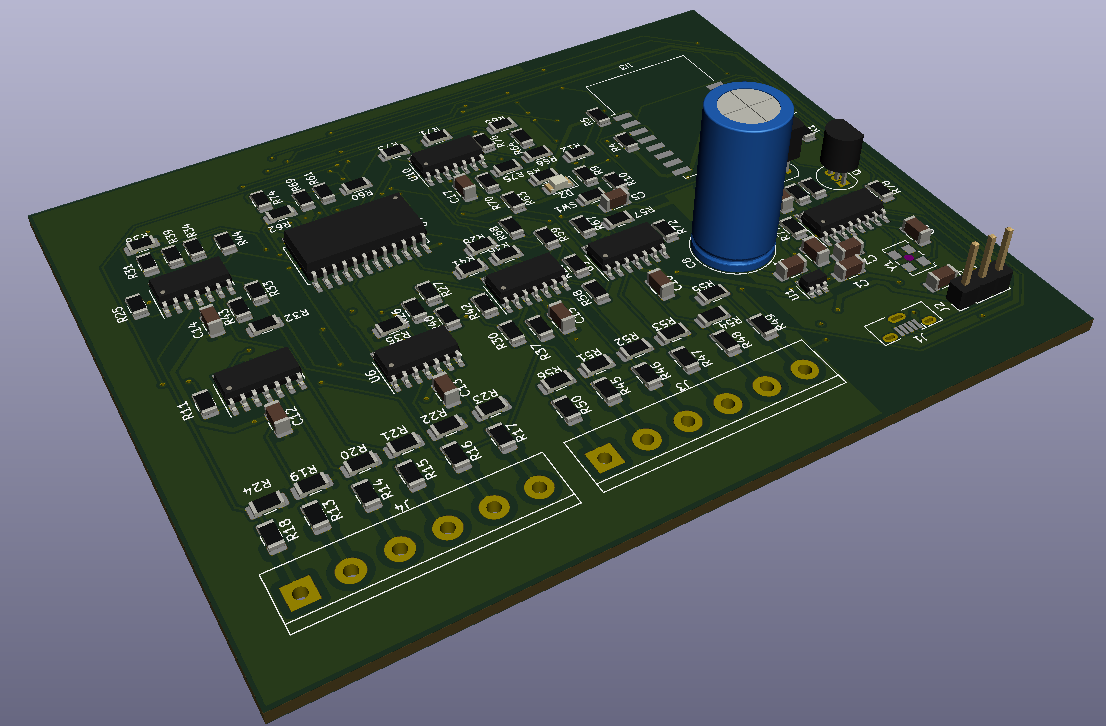
\includegraphics[scale=0.32]{images/3d_1.png}
\end{center}
\caption{Vista 3D de la cara superior de la placa}
\label{fig:3d_sup}
\end{figure}

\noindent Es pot observar com tots els amplificadors operacionals tenen un condensador molt proper; aquest condensador és el condensador de desacoblament. Els que he escollit son de 100 nF, un valor molt típic.\\
\newline No es disposa del model 3D dels connectors de les senyals dels panells solars, del connector micro USB i del component ESP-12E.\\
\newline Pel que fa a la cara inferior, aquesta es mostra a la Figura \ref{fig:inf}.

\begin{figure}[H]
\begin{center}
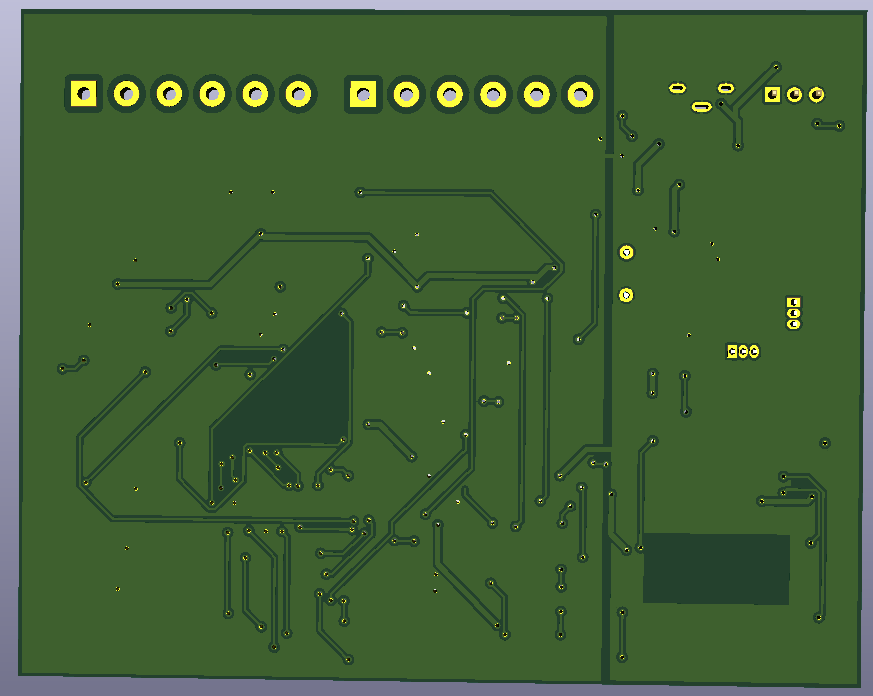
\includegraphics[scale=0.30]{images/3d_2.png}
\end{center}
\caption{Vista de la cara inferior de la placa}
\label{fig:inf}
\end{figure}
\noindent Els plans de massa es connecten per un petit conductor. D'aquesta manera el pla de massa digital està connectat al pla de massa de la part analògica del circuit i alhora es minimitza el soroll transmès de la part digital a l'analògica.


\clearpage


% Table generated by Excel2LaTeX from sheet 'Hoja1'
%\begin{table}[H]
%  \centering
%    \begin{tabularx} {\textwidth} {|X|r|} \hline
%  \multicolumn{1}{|c|}{Descripció} &  \multicolumn{1}{c|}{Quantitat}\\ \hline \hline
%
 %   Placa GLC 330 W & 10 \\ \hline
%    Inversor FRONIUS Primo 3.0-1 Light 3kW & 1 \\ \hline
%    Metres cable Ethernet RJ-45 CAT 8 & 10 \\ \hline
%    Metres cable 4 m$m^2$ PVC & 45 \\ \hline
 %   Metres cable 1,5 m$m^2$ PVC & 100 \\ \hline
 %   Punteres Enghofer E 4-10, 4 m$m^2$, 10 mm & 20 \\ \hline
 %   Punteres Enghofer E 1.5-10 1,5 m$m^2$ 10 mm & 12 \\ \hline
 %   Cinta aïllant 10 m 1,6 cm & 3 \\ \hline
 %   Caixa estanca Solera CONS 100x100x55 mm & 2 \\ \hline
  %  Canal Euroquint 25,16 mm 1,5 metres & 20 \\ \hline
%    Curva canal VECAMCO & 10 \\ \hline
%    Paquet de 50 brides 200x2,6  mm & 2 \\ \hline
%    Regleta nylon 12 pols 16 mm & 4 \\ \hline
%    Premsaestopes M12 & 10 \\ \hline
%    Cargol autoroscant M4 16 mm & 12 \\ \hline
%    Tacs Fischer 072095 nylon 6x50 mm & 50 \\ \hline
%    Díode SM74611KTTR & 10 \\ \hline
%            Hores enginyer & 1 \\ \hline
%    Hores oficial de primera & 12 \\ \hline
%    Hores oficial de segona & 12 \\ \hline
%    \end{tabularx}%
%  \label{tab:addlabel}%
% \end{table}%
